This section shows the results obtained with the TRITIUM-IFIC 1 prototype  during its installation in the IFIC laboratory. Several improvements, such as a Teflon vessel and new straight arrangement of scintillating fibers, was included in the design of this prototype, which were found to be problematic for the previous prototype, reducing its efficiency.

The signal and background energy spectra are shown in Figure \ref{subfig:SignalBackgroundEnergySpectraTritiumIFIC1}. The difference between both energy spectra corresponds to the tritium energy spectrum, Figura \ref{subfig:TritiumEnergySpectraTritiumIFIC1}. Furthermore, the tritium detection efficiency of this prototype was improved compared to TRITIUM-IFIC 0 prototype. This improvement can be quantified as in the previous section. The rate measured are given in Table \ref{tab:CountsPerSecondTRITIUMIFIC1}, where the tritium counts are obtained from the difference of signal and background spectra.

\begin{figure}
\centering
    \begin{subfigure}[b]{1\textwidth}
    \centering
    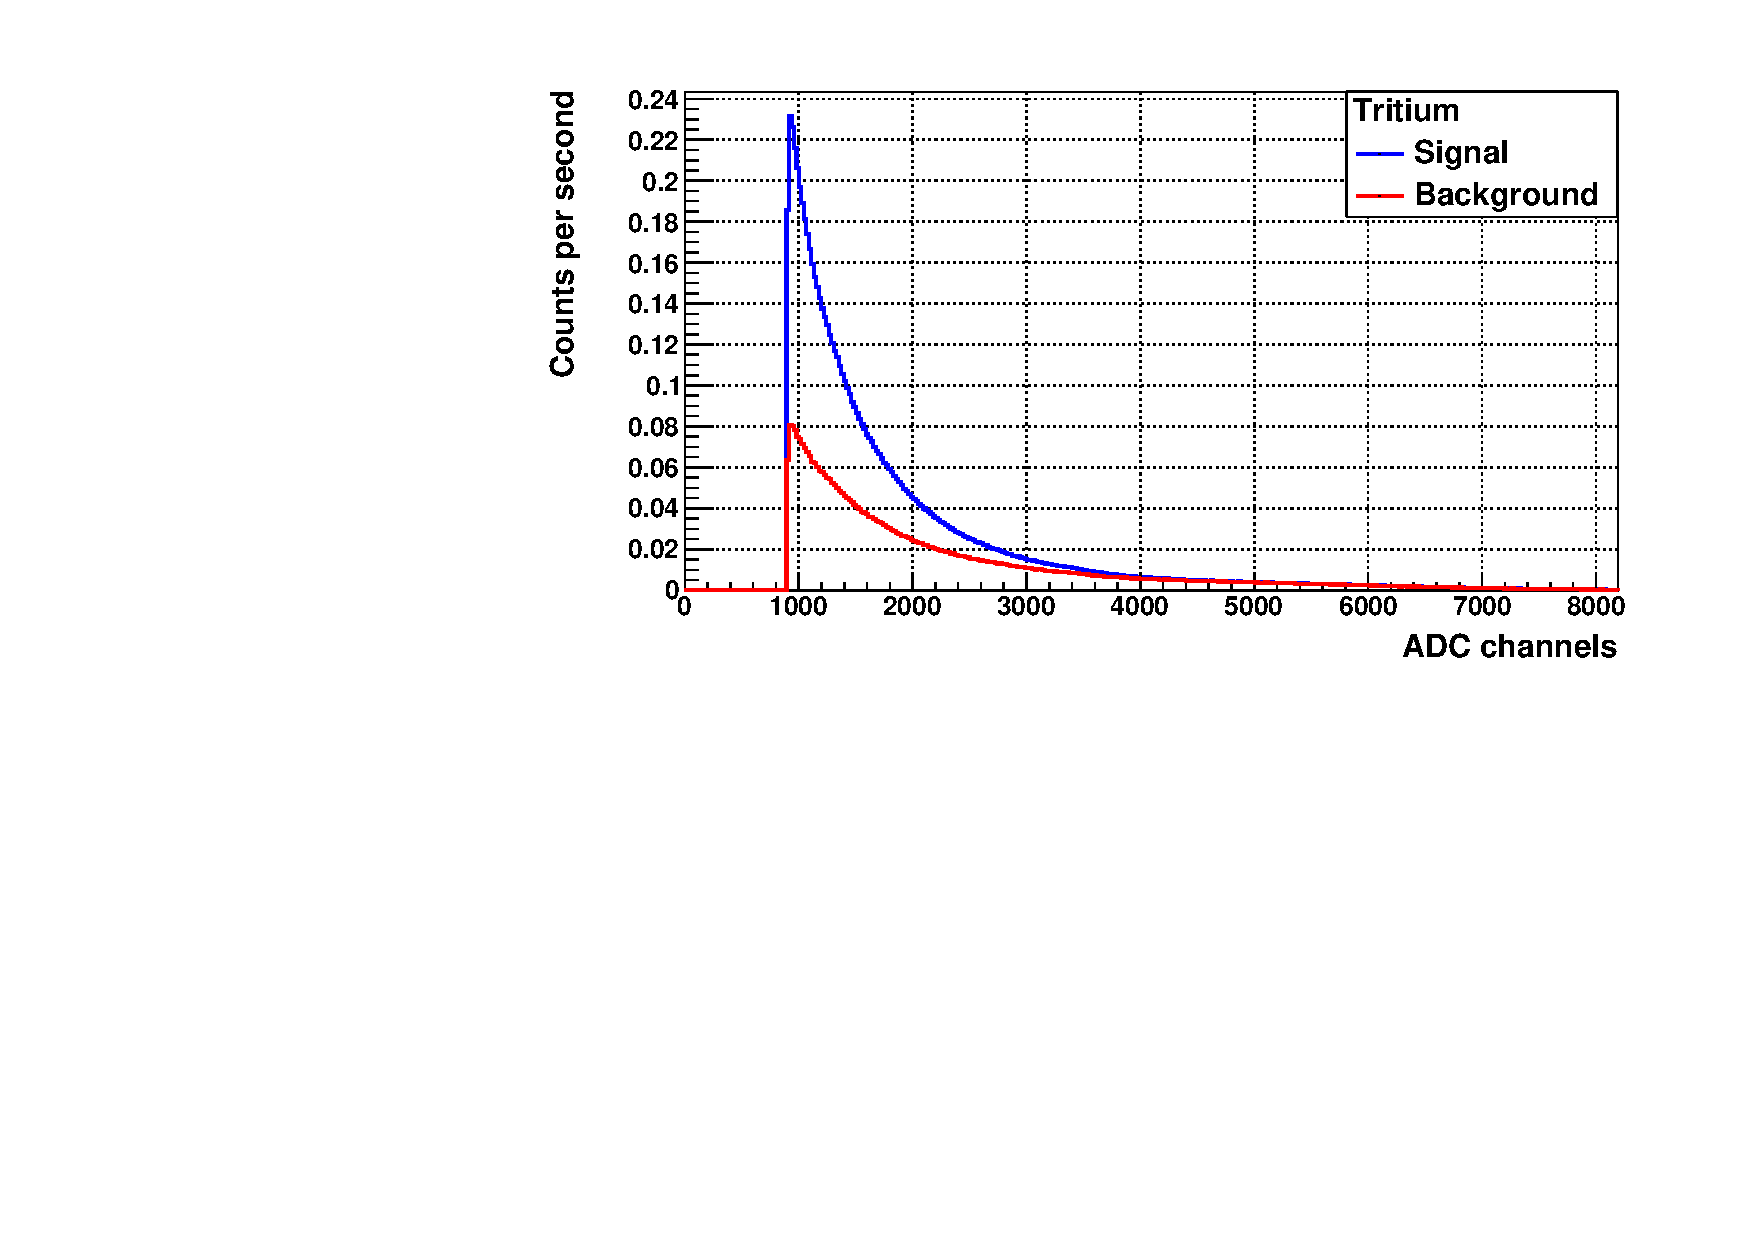
\includegraphics[width=\textwidth]{7ExperimentalResultsDetectors/71ExperimentalResultsLaboratory/712TRITIUMIFIC1/TritiumIFIC1Signals.pdf}  
    \caption{\label{subfig:SignalBackgroundEnergySpectraTritiumIFIC1}}
    \end{subfigure}
    \hfill
    \begin{subfigure}[b]{1\textwidth}
    \centering
    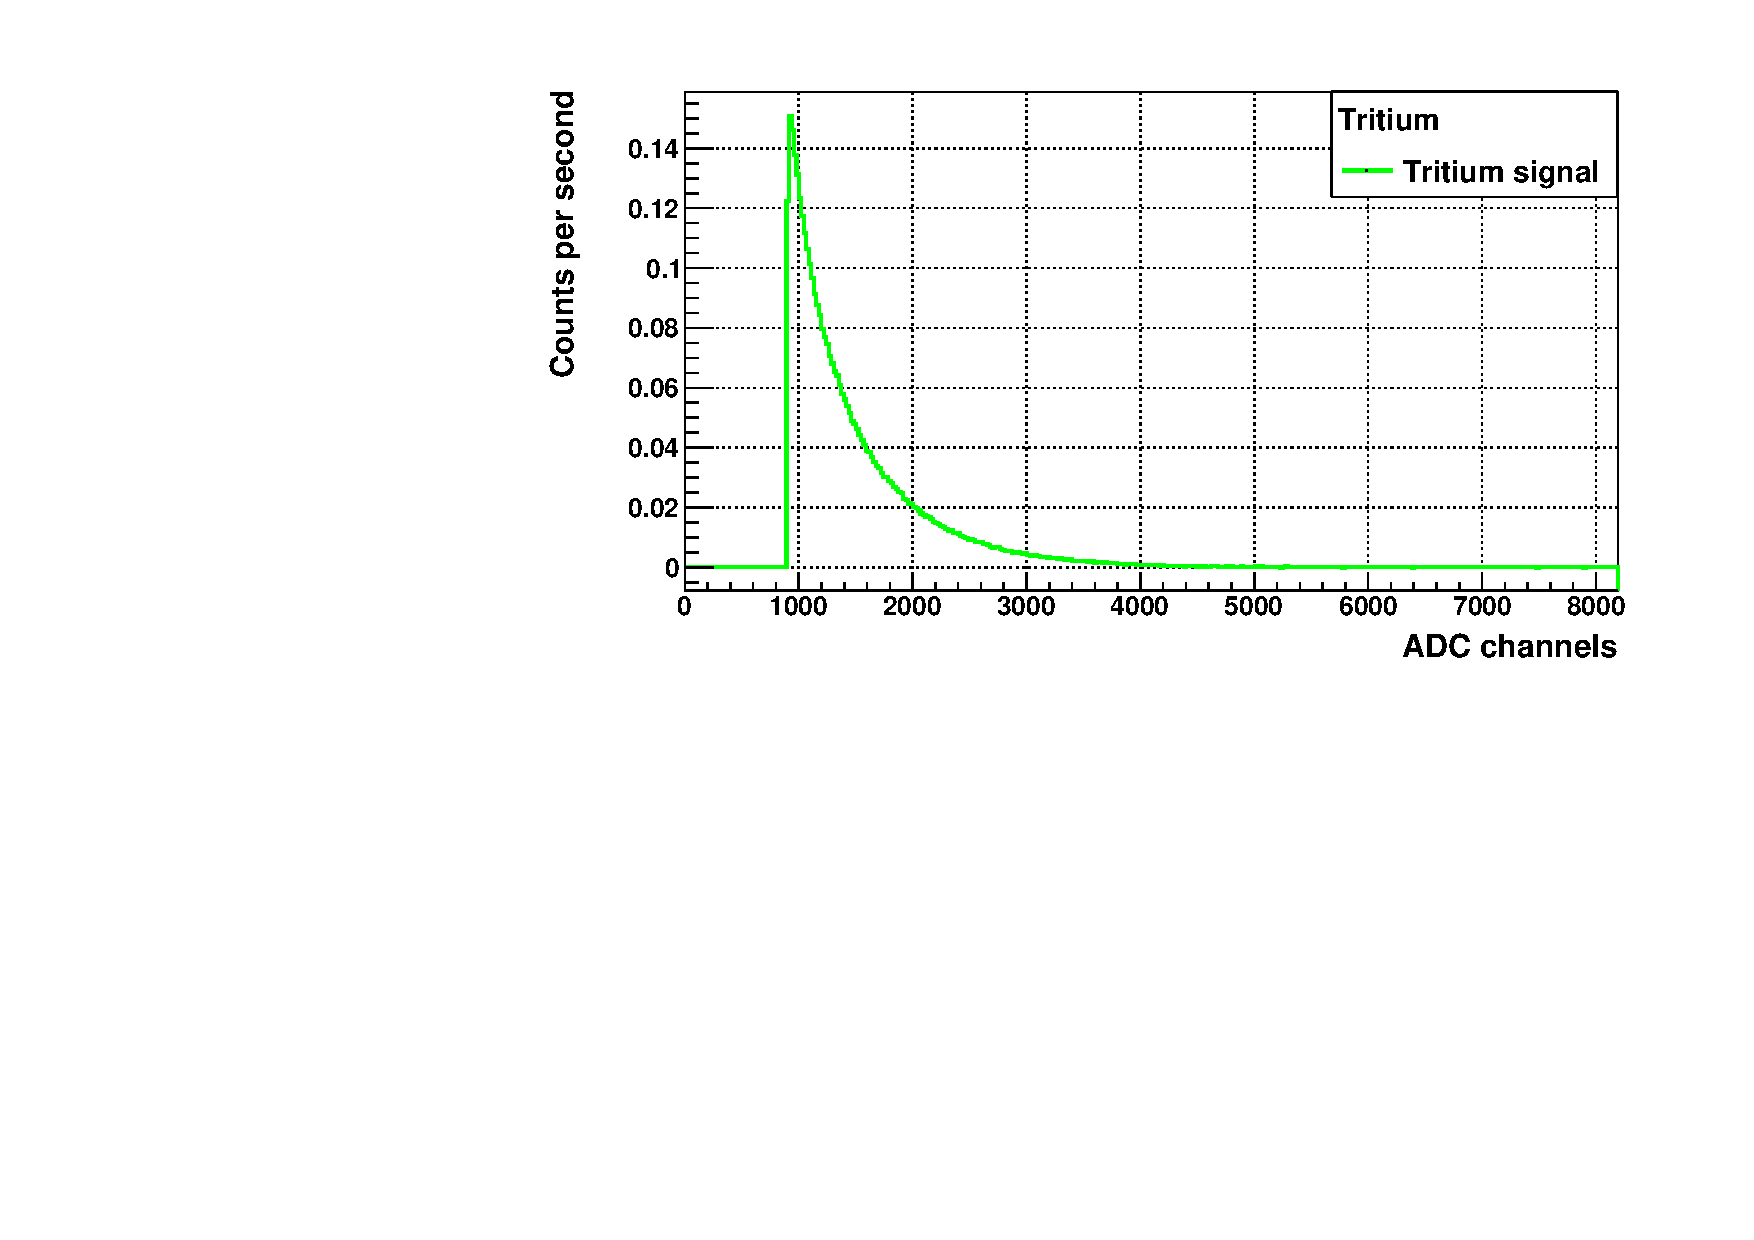
\includegraphics[width=\textwidth]{7ExperimentalResultsDetectors/71ExperimentalResultsLaboratory/712TRITIUMIFIC1/TritiumIFIC1Clear.pdf}  
    \caption{\label{subfig:TritiumEnergySpectraTritiumIFIC1}}
    \end{subfigure}
 \caption{Energy spectra measured with TRITIUM-IFIC 1 prototype. a) Signal and background energy spectra. b) Tritium energy spectrum.}
 \label{fig:EnergySpectraTRITIUMIFIC1}
\end{figure}

\begin{table}[h]
%%\centering
\begin{center}
\begin{tabular}{|c|c|}
\hline
Spectrum & Counts/second\\
\hline \hline \hline
Signal prototype & $7.82 \pm 0.11$ \\ \hline
Background prototype & $3.99 \pm 0.08$ \\ \hline
Tritium counts & $3.83 \pm 0.13$ \\ \hline
\end{tabular}
\caption{Counting rate obtained with the TRITIUM-IFIC 1 prototype.}
\label{tab:CountsPerSecondTRITIUMIFIC1}
\end{center}
\end{table}

The tritium detection efficiency obtained for TRITIUM-IFIC 1 is $(3.84 \pm 0.16)\cdot{} 10^{-2}~\liter\second^{-1}\kilo\becquerel^{-1}$. The efficiency obtained for this prototype is larger than that of TRITIUM-IFIC 0, as expected since this prototype has a larger active area. The specific efficiency obtained is $(9.56 \pm 0.40)\cdot{} 10^{-5}~\liter\second^{-1}\kilo\becquerel^{-1}\cm^{-2}$, which is a factor of ten better than that of TRITIUM-IFIC 0. Furthermore, compared to scintillating detectors developed in other experiments, table \ref{tab:PlasticScinTritium}, the efficiency of this prototype is very close to the best result, obtained by Singh, and the specific efficiency, which is the most relevant parameter to compare, is almost 5 times larger than that obtained by Hofstetter \cite{Hofstetter1, Hofstetter2}.

%It must be taken into account that in the first two prototypes the Low Detection Level, LDL, was not studied, since their objective was to improve its design and find the problems that reduced their efficiency. In fact, it can be seen in Figure \ref{fig:EnergySpectraTRITIUMIFIC1} that the activity used is further to be the LDL of the TRITIUM-IFIC 1 prototype. The LDL was only studied in the final prototypes.